\section{Model}

\subsection{Social Media}

\subsubsection{Machine Learning}

Sarker et al.~\cite{sarker2016social} proposed a stacking based ensemble classifier to automatically detect whether tweets are abuse or not when they contain specific 4 medication names. The architecture of the methodology is shown in figure~\ref{fig:model-sarker}. In the ensemble classifier, they used four algorithms - naive bayes (NB), SVM, maximum entropy (ME), and J48, and used various features such as n-gram, abuse-indicating terms, lexicon matches, synonym expansion, word cloud. They concluded that tweets are often ambiguous and impersonal, and a large number of corpus needed for better results. A sample of their annotated data is available~\footnote{\url{http://diego.asu.edu/Publications/DrugAbuse_DrugSafety.html}}. 

\begin{figure}[h]
	\centering
	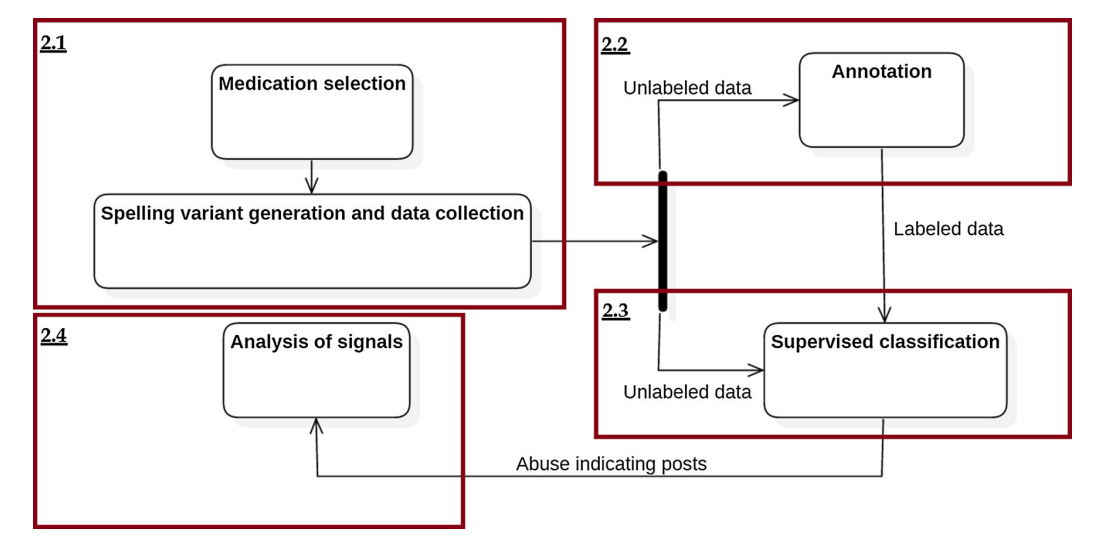
\includegraphics[width=0.99\linewidth]{Figures/h.png}
	\caption{Architecture by Sarker et al.~\cite{sarker2016social}}
	\label{fig:model-sarker}
\end{figure}

Alvaro et al.~\cite{alvaro2015crowdsourcing} explored whether tweets contains information about first-hand medication user experience. The structure of their model is elucidated in figure~\ref{fig:flowchart-alvaro}. They used a couple of algorithms - C50, SVM, NB, Multi-Layer Perceptron (MLP), Generalized Linear Model (GLM), and Bayesian Generalized Linear Model (BGLM). In their experiment, BGLM achieved highest F1-score for almost all sets of features.

\begin{figure}[h]
	\centering
	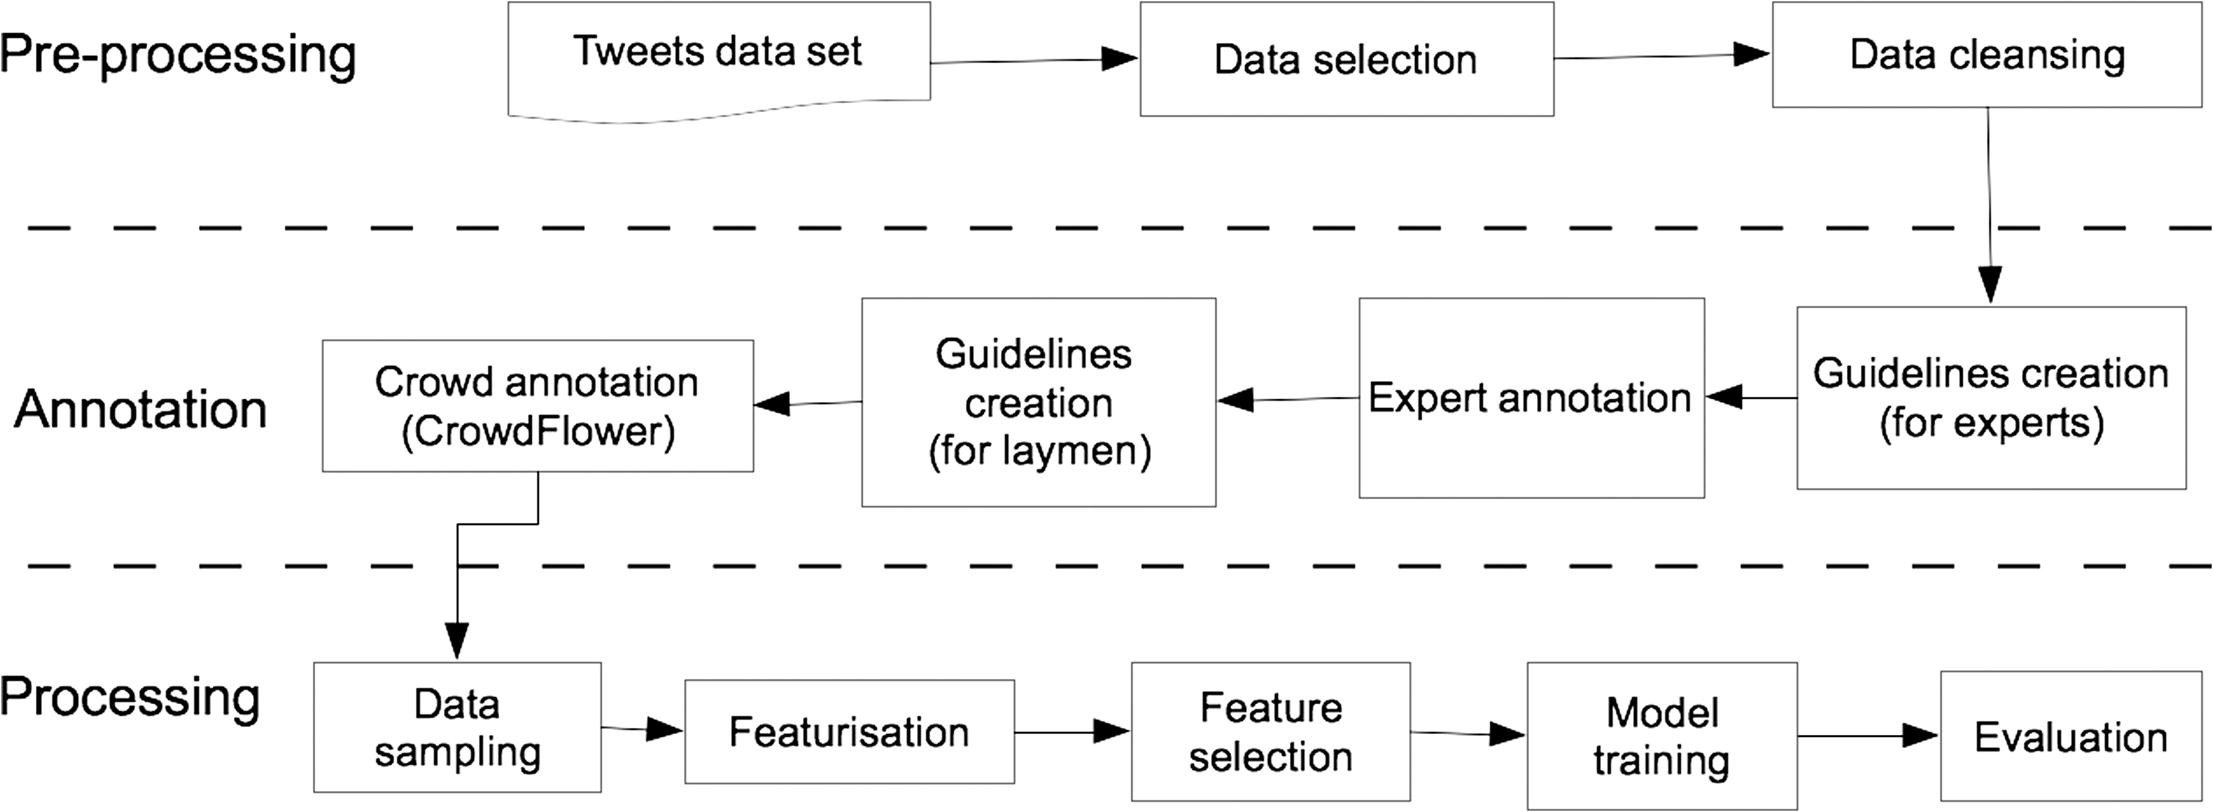
\includegraphics[width=0.99\linewidth]{Figures/n.jpg}
	\caption{Flow chart of Alvaro et al.~\cite{alvaro2015crowdsourcing}’s methodology.}
	\label{fig:flowchart-alvaro}
\end{figure}

Meanwhile, to detect a tweet contains ADR or not, Zhang et al.~\cite{zhang2016ensemble} applied an ensemble algorithm of four classifiers: (1) a concept-matching classifier based on ADR lexicon; (2) a ME classifier with word-level n-gram features and TFIDF weighting scheme; (3) a ME classifier based on word-level n-grams using NB log count ratios as feature values; and (4) a ME classifier with word embedding features. They obtain an F1-score of 0.4182 (positive class). The code of their model is available~\footnote{\url{https://github.com/tjflexic/psb-adr}}.

\subsubsection{Deep Learning}

However, these approaches~\cite{sarker2016social, alvaro2015crowdsourcing, zhang2016ensemble} heavily rely on feature engineering and require large amount of expert knowledge. Recently the focus has shifted towards deep learning. Tutubalina et al.~\cite{TUTUBALINA201893} proposed a model based on bidirectional RNN for MCN in social media. The architecture is illustrated in figure~\ref{fig:architecture-tutubalina}.

\begin{figure}[h]
	\centering
	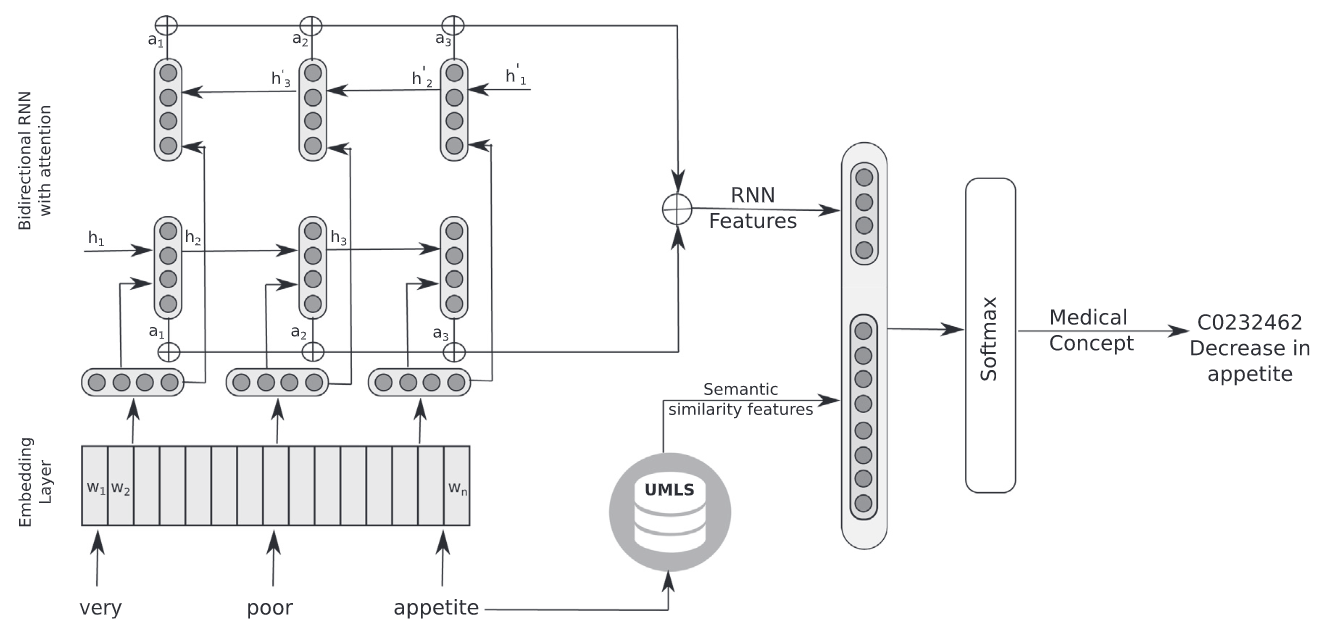
\includegraphics[width=0.99\linewidth]{Figures/f.png}
	\caption{Architecture for MCN in social media by Tutubalina et al.~\cite{TUTUBALINA201893}.}
	\label{fig:architecture-tutubalina}
\end{figure}

Huynh et al.~\cite{huynh2016adverse} investigated different neural network (NN) architecture for ADR classification. In particular, they applied their data over four algorithms: CNN, Recurrent Convolutional Neural Network (RCNN), Convolutional Recurrent Neural Network (CRNN), Convolutional Neural Network with Attention (CNNA). The architecture of these algorithms are shown in the figure 7. They compare model against Zhang et al.~\cite{zhang2016ensemble}’s model and found that CNN obtain highest F1-score. The source code of the project is available~\footnote{\url{https://github.com/trunghlt/AdverseDrugReaction}}.

\begin{figure}[h]
	\centering
	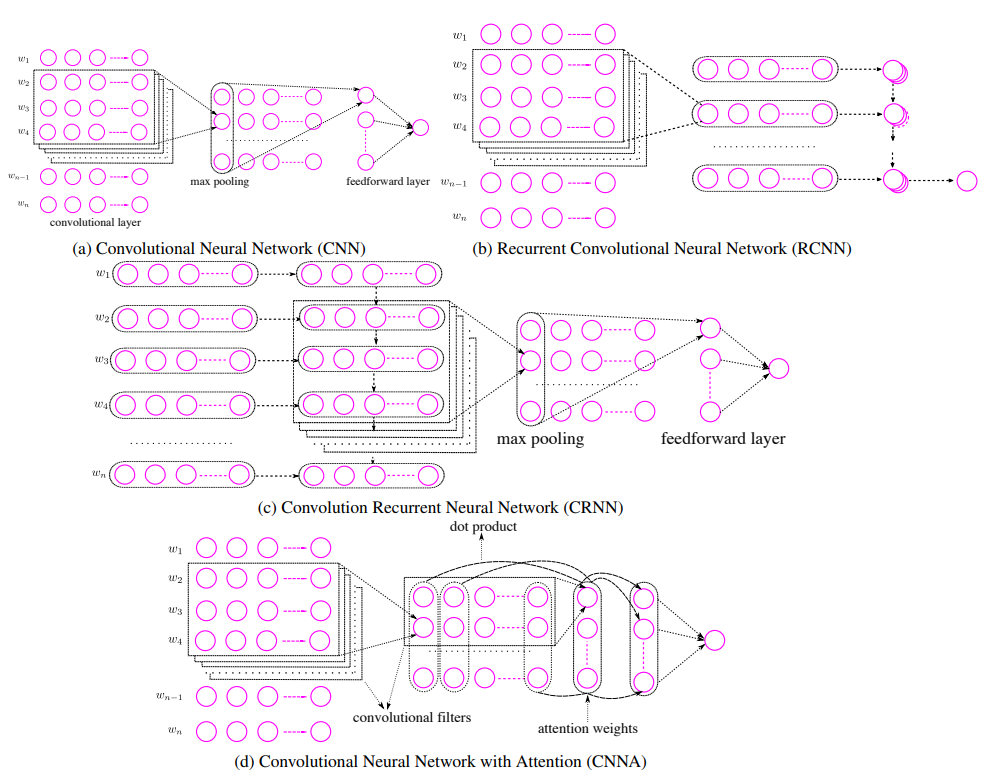
\includegraphics[width=0.99\linewidth]{Figures/e.png}
	\caption{Architecture by Huynh et al.~\cite{huynh2016adverse}.}
	\label{fig:architecture-huynh}
\end{figure}

Lee et al.~\cite{lee2017adverse}, meanwhile, applied a semi-supervised CNN framework for the same task. This model was developed by Johnson et al.~\cite{johnson2015semi}. Lee et al. found that this model outperform a strong state-of-the-art supervised classification model by +9.9\% F1-score. The architecture of the model is shown in the figure~\ref{fig:architecture-lee}. The method works in two phases: (1) unsupervised phrase embedding learning, and (2) integrating the learned embeddings into the supervised training that uses labeled data.

\begin{figure}[h]
	\centering
	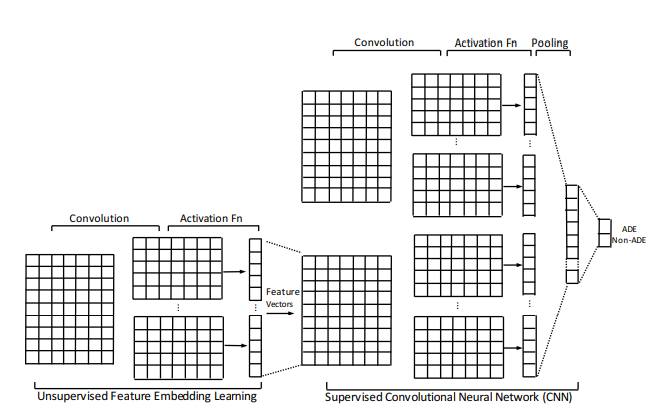
\includegraphics[width=0.99\linewidth]{Figures/l.png}
	\caption{Semi-supervised CNN by Lee et al.~\cite{lee2017adverse}.}
	\label{fig:architecture-lee}
\end{figure}

Weissenbacher et al.~\cite{weissenbacher2019deep} introduced a deep neural networks ensemble method - \textit{Kusuri} - a LSTM model - to detect medication names in unbalanced tweets. \textit{Kusuri} is composed of two modules: first, applied four different classifiers (lexicon based, spelling variant based, pattern based, and a weakly trained neural network) parallel to discover potential tweets with medication names; second, an ensemble of deep neural networks encoding morphological, semantic, and longrange dependencies of important words in the tweets makes the final decision. The architecture is shown in figure~\ref{fig:architecture-weissenbacher}. This model achieves an F1-score of 0.788 on an extremely unbalanced dataset (98959 tweets, with only 0.26\% mentioning medications). A brief description of four algorithms are provided by the authors~\footnote{\url{https://tinyurl.com/y47qzbcq}}.

\begin{figure}[h]
	\centering
	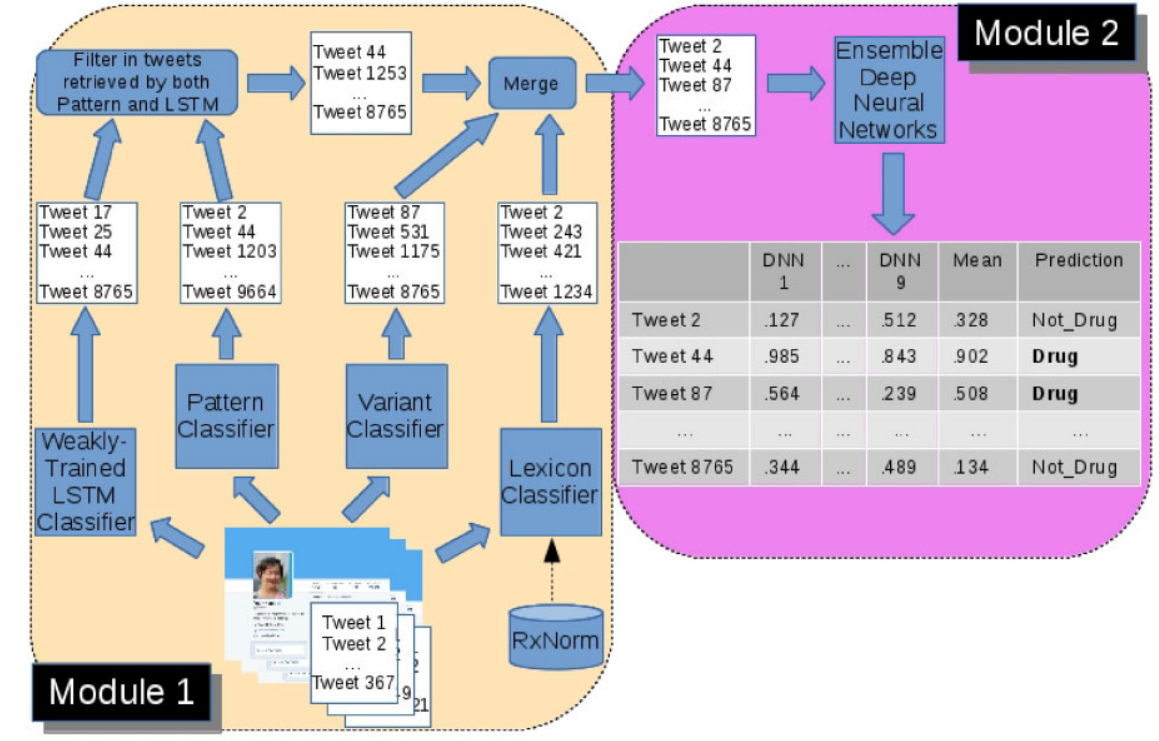
\includegraphics[width=0.99\linewidth]{Figures/a.png}
	\caption{\textit{Kusuri} model by Weissenbacher et al.~\cite{weissenbacher2019deep}.}
	\label{fig:architecture-weissenbacher}
\end{figure}

Wu et al.~\cite{wu2019msa} proposed neural approach using multi-head self-attention (MSA) to jointly detect drug name and adverse drug reaction. Their MSA model has three modules: first, a word representation module, which aims to build the contextual representations of words from the original characters within them; second, a tweet representation module; third, a classification module. The framework of the model is illustrated in the figure~\ref{fig:architecture-wu-msa}.

\begin{figure}[h]
	\centering
	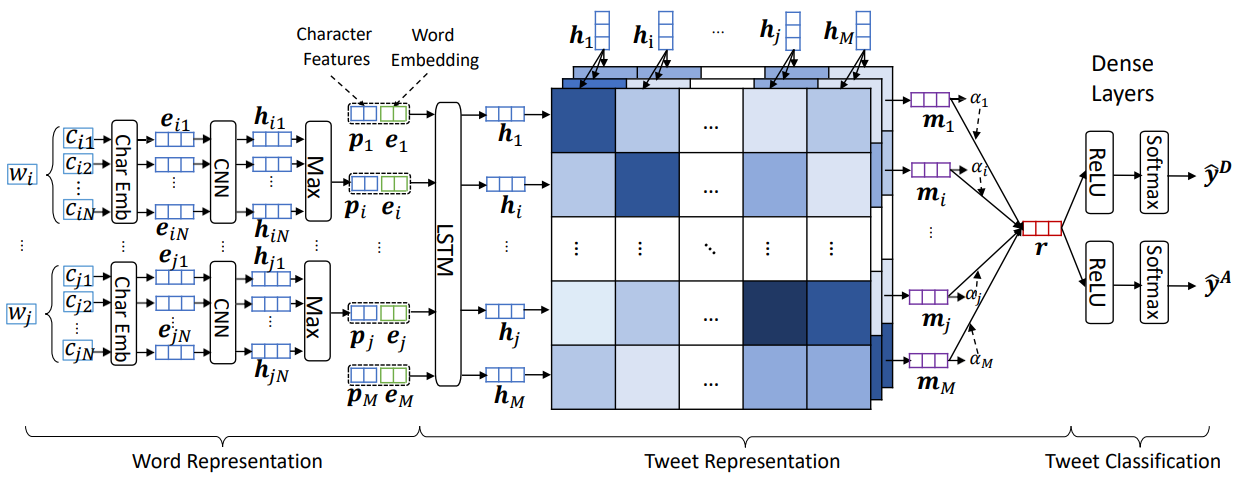
\includegraphics[width=0.99\linewidth]{Figures/k.png}
	\caption{MSA model by Wu et al.~\cite{wu2019msa}.}
	\label{fig:architecture-wu-msa} 
\end{figure}

\subsection{Clinical Texts and Health Records}

Researches has been conducted thoroughly to extract medication names from clinical texts and health records~\cite{weeks2020medextractr, kim2020ensemble, ju2020ensemble}. 2018 n2c2 shared task on adverse drug events and medication extraction~\footnote{\url{https://portal.dbmi.hms.harvard.edu/projects/n2c2-2018-t2/}}, Kim et al.~\cite{kim2020ensemble} demonstrated that a stacked ensemble with a search-based structured prediction algorithm achieved good performance (an F1 score of 0.9266 on official dataset) by effectively integrating the output of individual classifiers. Their architecture is shown in figure~\ref{fig:architecture-kim}.

\begin{figure}[h]
	\centering
	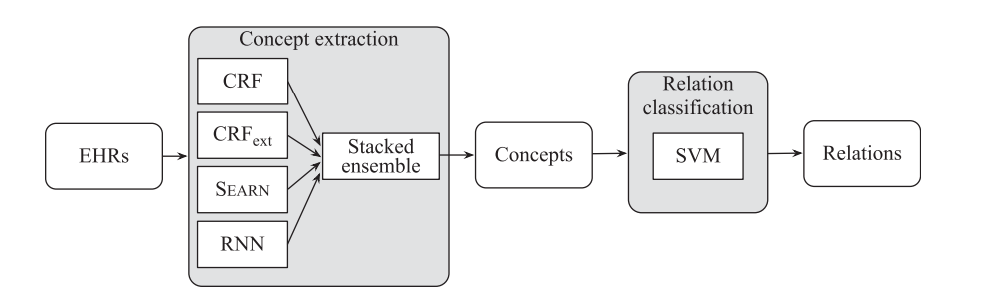
\includegraphics[width=0.99\linewidth]{Figures/i.png}
	\caption{Framework of model by Kim et al.~\cite{kim2020ensemble}.}
	\label{fig:architecture-kim}
\end{figure}

Ju et al.~\cite{ju2020ensemble} proposed an ensembling system based on neural network to automatically extract adverse drug events and drug related entities from clinical narratives. They firstly pre-processed Electronic Health Records(EHR) using sentence segmentation and tokenization. Then they implemented feature based and neural network-based models to detect ADEs and related medications. The architecture is shown in figure~\ref{fig:architecture-ju}. Their method achieved 92.78\% lenient micro F1-score, with 95.99\% lenient precision, and 89.79\% lenient recall.

\begin{figure}[h]
	\centering
	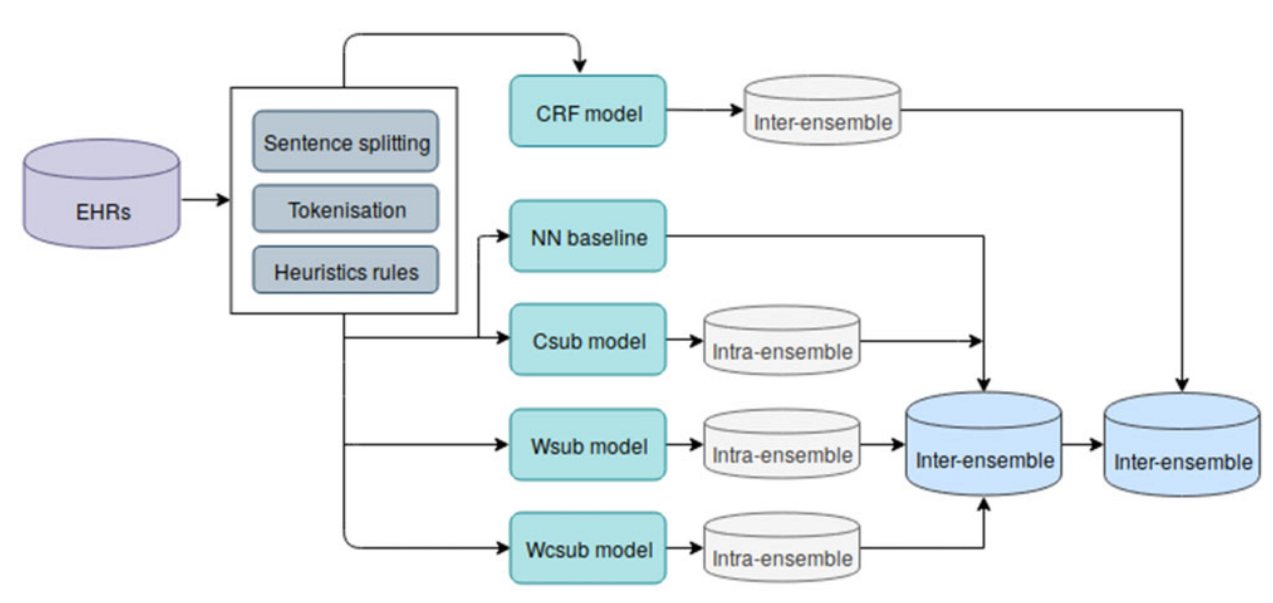
\includegraphics[width=0.99\linewidth]{Figures/c.png}
	\caption{Framework of model by Ju et al.~\cite{ju2020ensemble}.}
	\label{fig:architecture-ju}
\end{figure}

The research of extracting medication names in other languages has been an area of interest as well. Armengol-Estape et al.~\cite{armengol2019pharmaconer} proposed a deep learning-based tool for automatically finding chemicals and drugs in Spanish medical texts.